






\vspace{-3mm}
\section{Defenses}
\vspace{-2mm}
Many defenses~\cite{steinhardt2017certified,wang2019neural,jia2021intrinsic,jia2022certified,jia2023pore,wang2024fcert} were proposed to defend against data poisoning attacks that compromise the training dataset of a machine learning model. However, most of them are not applicable since {\name} does not compromise the training dataset of an LLM. \RV{Another defense is to (manually) check retrieved texts when observing generation error~\cite{shan2022poison}. However, the generation error could also happen for many other reasons, making this solution time-consuming and less practical.}
Thus, we generalize some widely used defenses against  attacks~\cite{jain2023baseline, alon2023detecting, gonen2022demystifying} to LLM to defend against {\name}.

\vspace{-3mm}
\subsection{Paraphrasing} 
Paraphrasing~\cite{jain2023baseline} was used to defend against prompt injection attacks~\cite{liu2023prompt, liuyi2023prompt, pedro2023prompt, branch2022evaluating} and jailbreaking attacks~\cite{wei2023jailbroken, zou2023universal, deng2023jailbreaker, qi2023visual, li2023multistep, shen2023do} to LLMs. We extend paraphrasing to defend against {\name}. In particular, given a text, the paraphrasing defense utilizes an LLM to paraphrase it. In our scenario, given a question, we use an LLM to paraphrase it before retrieving relevant texts from the knowledge database to generate an answer for it. Recall that {\name} crafts malicious texts such that they could be retrieved for a target question. For instance, in the black-box setting, {\name} prepends the target question to a text $I$ to craft a malicious text. In the white-box setting, {\name} optimizes a malicious text such that a retriever produces similar feature vectors for the malicious text and the target question. Our insight is that paraphrasing the target question would change its structure. For instance, when the target question is ``Who is the CEO of OpenAI?''. The paraphrased question could be ``Who holds the position of Chief Executive Officer at OpenAI?''. As a result, malicious texts may not be retrieved for the paraphrased target question. Note that we do not paraphrase texts in the knowledge database  
due to high computational costs.


\begin{table}[!t]\renewcommand{\arraystretch}{1.5}
\setlength{\tabcolsep}{1mm}
\fontsize{7.5}{8}\selectfont 
\centering
\caption{{\name} under paraphrasing defense.}
\vspace{-2mm}
\begin{tabular}{|c|c|c|c|c|c|}
\hline
  \multirow{2}{*}{Dataset} &\multirow{2}{*}{Attack} & \multicolumn{2}{c|}{w.o. defense} & \multicolumn{2}{c|}{with defense}    \\ \cline{3-6}
& &ASR&F1-Score&ASR&F1-Score \\ \hline
                      
\multirow{2}{*}{NQ}& {\name} (Black-Box)         & 0.97 & 0.96 & 0.87 & 0.83 \\ \cline{2-6}
& {\name} (White-Box)         &  0.97& 1.0 & 0.93 & 0.94\\ \hline \hline 
\multirow{2}{*}{HotpotQA}& {\name} (Black-Box)         &  0.99 & 1.0  & 0.93 & 1.0 \\ \cline{2-6}
& {\name} (White-Box)         &  0.94 & 1.0  & 0.86 & 1.0\\ \hline \hline 
\multirow{2}{*}{MS-MARCO}& {\name} (Black-Box)        &  0.91 & 0.89  & 0.79 & 0.70\\ \cline{2-6}
& {\name} (White-Box)      &  0.90 & 0.94  & 0.81 & 0.80 \\ \hline 

\end{tabular}
\label{tab:paraphrasing-defense}
\vspace{-5mm}
\end{table}


We conduct experiments to evaluate the effectiveness of paraphrasing defense. In particular, for each target question, we generate 5 paraphrased target questions using GPT-4, where the prompt can be found in Appendix~\ref{prompt-paraphrase-defense}. 
 For each paraphrased target question, we retrieve $k$ texts from the corrupted knowledge database (the malicious texts are crafted for the original target questions using {\name}). Then, we generate an answer for the paraphrased target question based on the $k$ retrieved texts. We adopt the same default setting as that in Section~\ref{sec:exp} (e.g., $k=5$ and 5 injected malicious texts for each target question). We report the ASR and F1-Score (note that Precision and Recall are the same as F1-Score under our default setting). ASR measures the fraction of paraphrased target questions whose answers are the corresponding attacker-chosen target answers. F1-Score is higher when more malicious texts designed for a target question are retrieved for the corresponding paraphrased target questions. Table~\ref{tab:paraphrasing-defense} shows our experimental results. We find that {\name} could still achieve high ASRs and F1-Score, which means paraphrasing defense cannot effectively defend against {\name}.






\vspace{-3mm}
\subsection{Perplexity-based Detection} Perplexity (PPL)~\cite{jelinek1980interpolated}  is widely used to measure the quality of texts, which is also utilized to defend against attacks to LLMs~\cite{jain2023baseline, alon2023detecting, gonen2022demystifying}. A large perplexity of a text means it is of low quality. We utilize perplexity to detect malicious texts. For instance, in the white-box setting, {\name} utilizes adversarial attacks to craft malicious texts, which may influence the quality of malicious texts. Thus, a text with lower text quality (i.e., high perplexity) is more likely to be malicious. 
 We calculate the perplexity for all clean texts in the database as well as all malicious texts crafted by {\name}. 
In our experiment, we use the cl100k\_base model from OpenAI tiktoken~\cite{tiktoken} to calculate perplexity. 

Figure~\ref{PPL_ROC_nq} shows the ROC curve as well as AUC. We find that the false positive rate (FPR) is also very large when the true positive rate (TPR) is very large. This means a large fraction of clean texts are also detected as malicious texts when malicious texts are detected, i.e., the perplexity values of malicious texts are not statistically higher than those of clean texts, which means it is very challenging to detect malicious texts using perplexity. We suspect the reasons are as follows. Recall that each malicious text $P$ is the concatenation of $S$ and $I$, i.e., $P=S \oplus I$. The sub-text $I$ 
is generated by GPT-4, which is of high quality. For {\name} in the black-box setting, $S$ is the target question, which is a normal text. As a result, the text quality of the malicious text is normal. 
We find that the AUC of {\name} in the white-box setting is slightly larger than that in the black-box setting, which means the text quality is influenced by the optimization but not substantially. 




\begin{figure}[!t]
\centering
{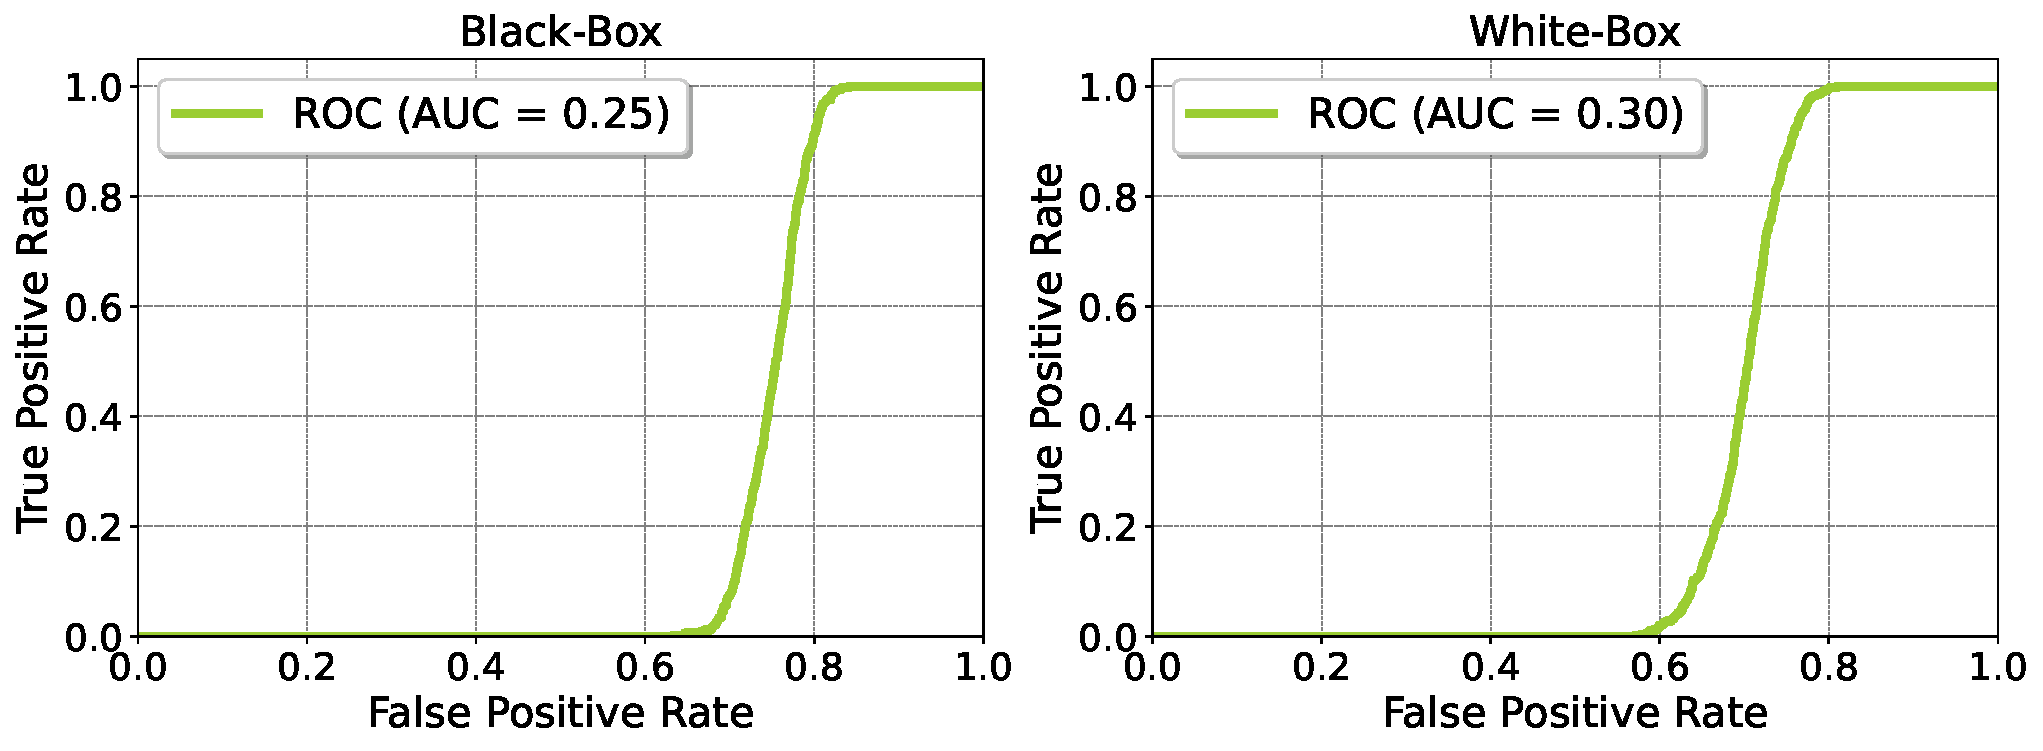
\includegraphics[width=0.45\textwidth]{figs/PPL_ROC_nq.pdf}}
\vspace{-2mm}
\caption{The ROC curves for PPL detection defense. The dataset is NQ. The results for other two datasets are in Figures~\ref{PPL_ROC_hotpotqa} and~\ref{PPL_ROC_msmarco} in Appendix.}
\label{PPL_ROC_nq}
\vspace{-5mm}
\end{figure}




\vspace{-3mm}
\subsection{Duplicate Text Filtering}
\label{sec:defense:duplicate}
{\name} generates each malicious text independently in both black-box and white-box settings. As a result, it is possible that some malicious texts could be the same. Thus, we could filter those duplicate texts to defend against {\name}. We add experiments to filter duplicate texts under the default setting in Section~\ref{sec:exp}. In particular, we calculate the hash value (using the SHA-256 hash function) for each text in a corrupted knowledge database and remove texts with the same hash value. Table~\ref{tab:dup-filter-defense} compares the ASR with and without defense. We find that the ASR is the same, which means duplicate text filtering cannot successfully filter malicious texts.  
The reason is that the sub-text $I$ (generated by GPT-4 in our experiment) in each malicious text is different, resulting in diverse malicious texts.


\begin{table}[!t]\renewcommand{\arraystretch}{1.5}
\setlength{\tabcolsep}{1mm}
\fontsize{7.5}{8}\selectfont 
\centering
\caption{The effectiveness of {\name} under duplicate text filtering defense.}
\vspace{-2mm}
\begin{tabular}{|c|c|c|c|c|c|}
\hline
  \multirow{2}{*}{Dataset} &\multirow{2}{*}{Attack} & \multicolumn{2}{c|}{w.o. defense} & \multicolumn{2}{c|}{with defense}    \\ \cline{3-6}
& &ASR&F1-Score&ASR&F1-Score \\ \hline
\multirow{2}{*}{NQ}& {\name} (Black-Box)         & 0.97 & 0.96 & 0.97 & 0.96 \\ \cline{2-6}
& {\name} (White-Box)          &  0.97 & 1.0  & 0.97 & 1.0 \\ \hline \hline 
\multirow{2}{*}{HotpotQA}& {\name} (Black-Box)  & 0.99 & 1.0  & 0.99 & 1.0 \\ \cline{2-6}
& {\name} (White-Box)         & 0.94 & 1.0 & 0.94 & 1.0 \\ \hline \hline 
\multirow{2}{*}{MS-MARCO}& {\name} (Black-Box)         & 0.91 & 0.89 & 0.91 & 0.89 \\ \cline{2-6}
& {\name} (White-Box)        & 0.90 & 0.94 & 0.90 & 0.94 \\ \hline 

\end{tabular}
\label{tab:dup-filter-defense}
\vspace{-4mm}
\end{table}

\vspace{-3mm}
\subsection{Knowledge Expansion}
{\name} injects at most $N$ malicious texts into a knowledge database for each target question. Thus, if we retrieve $k$ texts, with $k>N$, then it is very likely that $k-N$ texts would be clean ones. This inspires us to retrieve more texts to defend against {\name}. We call this defense \emph{Knowledge Expansion}. We conduct experiments under the default setting, where $N=5$. Figures~\ref{Big_k_nq}, \ref{Big_k_hotpotqa}, \ref{Big_k_msmarco} (in Appendix) shows the ASRs, Precision, Recall, and F1-Score for large $k$. We find that this defense still cannot completely defend against our {\name} even if $k=50$ (around 10\% retrieved texts are malicious ones when injecting $N=5$ malicious texts for each target question). For instance, {\name} could still achieve 41\% (black-box) and 43\% (white-box) ASR on HotpotQA when $k=50$. Additionally, we find that ASR further increases as $N$ increases (shown in Figures~\ref{Big_N_nq}, \ref{Big_N_hotpotqa}, \ref{Big_N_msmarco} in Appendix), which means this defense is less effective when an attacker could inject more malicious texts into the knowledge database. We note that this defense also incurs large computation costs for an LLM to generate an answer due to the long context (caused by more retrieved texts).  


